\documentclass[hidelinks,12pt]{article}
\usepackage[left=0.25cm,top=1cm,right=0.25cm,bottom=1cm]{geometry}
%\usepackage[landscape]{geometry}
\textwidth = 20cm
\hoffset = -1cm
\usepackage[utf8]{inputenc}
\usepackage[spanish,es-tabla]{babel}
\usepackage[autostyle,spanish=mexican]{csquotes}
\usepackage[tbtags]{amsmath}
\usepackage{nccmath}
\usepackage{amsthm}
\usepackage{amssymb}
\usepackage{mathrsfs}
\usepackage{graphicx}
\usepackage{subfig}
\usepackage{standalone}
\usepackage[outdir=./Imagenes/]{epstopdf}
\usepackage{siunitx}
\usepackage{physics}
\usepackage{color}
\usepackage{float}
\usepackage{hyperref}
\usepackage{multicol}
%\usepackage{milista}
\usepackage{anyfontsize}
\usepackage{anysize}
%\usepackage{enumerate}
\usepackage[shortlabels]{enumitem}
\usepackage{capt-of}
\usepackage{bm}
\usepackage{relsize}
\usepackage{placeins}
\usepackage{empheq}
\usepackage{cancel}
\usepackage{wrapfig}
\usepackage[flushleft]{threeparttable}
\usepackage{makecell}
\usepackage{fancyhdr}
\usepackage{tikz}
\usepackage{bigints}
\usepackage{scalerel}
\usepackage{pgfplots}
\usepackage{pdflscape}
\pgfplotsset{compat=1.16}
\spanishdecimal{.}
\renewcommand{\baselinestretch}{1.5} 
\renewcommand\labelenumii{\theenumi.{\arabic{enumii}})}
\newcommand{\ptilde}[1]{\ensuremath{{#1}^{\prime}}}
\newcommand{\stilde}[1]{\ensuremath{{#1}^{\prime \prime}}}
\newcommand{\ttilde}[1]{\ensuremath{{#1}^{\prime \prime \prime}}}
\newcommand{\ntilde}[2]{\ensuremath{{#1}^{(#2)}}}

\newtheorem{defi}{{\it Definición}}[section]
\newtheorem{teo}{{\it Teorema}}[section]
\newtheorem{ejemplo}{{\it Ejemplo}}[section]
\newtheorem{propiedad}{{\it Propiedad}}[section]
\newtheorem{lema}{{\it Lema}}[section]
\newtheorem{cor}{Corolario}
\newtheorem{ejer}{Ejercicio}[section]

\newlist{milista}{enumerate}{2}
\setlist[milista,1]{label=\arabic*)}
\setlist[milista,2]{label=\arabic{milistai}.\arabic*)}
\newlength{\depthofsumsign}
\setlength{\depthofsumsign}{\depthof{$\sum$}}
\newcommand{\nsum}[1][1.4]{% only for \displaystyle
    \mathop{%
        \raisebox
            {-#1\depthofsumsign+1\depthofsumsign}
            {\scalebox
                {#1}
                {$\displaystyle\sum$}%
            }
    }
}
\def\scaleint#1{\vcenter{\hbox{\scaleto[3ex]{\displaystyle\int}{#1}}}}
\def\bs{\mkern-12mu}


%\author{M. en C. Gustavo Contreras Mayén. \texttt{curso.fisica.comp@gmail.com}}
\title{Transformada Discreta de Fourier \\ {\large Matemáticas Avanzadas de la Física}}
\date{ }
\begin{document}
\maketitle
\fontsize{14}{14}\selectfont
\section{Transformadas discreta de Fourier.}
El análisis de Fourier debe su nombre a Jean Baptiste Joseph Fourier (1768-1830), él estaba interesado en la
propagación del calor, y en 1807 publicó un artículo sobre como usar senoidales para representar distribuciones de temperatura, allí aseguró que cualquier señal periódica podría representarse como la suma de ondas senoidales, escogidas correctamente.
\par
Una señal puede ser continua o discreta, y puede ser periódica o aperiódica. La combinación de estas dos características genera las cuatro categorías, que se describen a continuación y se ilustran:
\begin{enumerate}
\item \textbf{No periódico-Continuo.}

Esto incluye, por ejemplo, exponenciales que decaen y la curva gaussiana. Estas señales se extienden de $(-\infty, \infty)$sin repetirse en un patrón periódico. La Transformada de Fourier para este tipo de señal se llama simplemente Transformada de Fourier.
\begin{figure}[H]
    \centering
    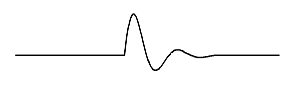
\includegraphics{Imagenes/TDF_01.png}
    \caption{Señal no periódica y continua: Transformada de Fourier.}
    \label{fig:figura_TDF_01}
\end{figure}
\item \textbf{Periódico-Continuo.}

Aquí, los ejemplos incluyen: ondas senoidales, ondas cuadradas y cualquier forma de onda que se repita en un patrón regular en $(-\infty, \infty)$. Esta versión de la transformada de Fourier se llama la Serie de Fourier.
\begin{figure}[H]
    \centering
    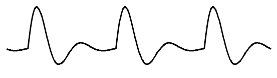
\includegraphics{Imagenes/TDF_02.png}
    \caption{Señal periódica y continua: Serie de Fourier.}
    \label{fig:figura_TDF_02}
\end{figure}
\item \textbf{No periódico-discreto.}

Estas señales solo se definen en puntos discretos en el dominio $(-\infty, \infty)$, y no se repiten de forma periódica. Este tipo de transformada de Fourier se denomina Transformada de Fourier en tiempo discreto.
\begin{figure}[H]
    \centering
    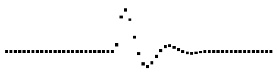
\includegraphics{Imagenes/TDF_03.png}
    \caption{Señal no periódica y discreta: Transformada de Fourier en tiempo discreto.}
    \label{fig:figura_TDF_03}
\end{figure}
\item \textbf{Periódico-Discreto.}

Estas son señales discretas que se repiten de manera periódica en el intervalo $(-\infty, \infty)$. Esta clase de Transformada de Fourier a veces se denomina Serie Discreta de Fourier, pero a menudo se denomina Transformada Discreta de Fourier.
\begin{figure}[H]
    \centering
    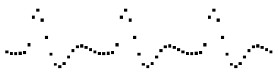
\includegraphics{Imagenes/TDF_04.png}
    \caption{Señal periódica y discreta: Transformada discreta de Fourier.}
    \label{fig:figura_TDF_04}
\end{figure}
\end{enumerate}
Estas cuatro clases de señales se extienden de $(-\infty. \infty)$ ¿Qué sucede si solo tiene un número finito de muestras almacenadas en la computadora?, digamos una señal formada a partir de $1024$ puntos. ¿No hay una versión de la Transformada de Fourier que use señales de longitud finita? No, no hay. Las ondas seno y coseno se definen como la extensión desde el infinito negativo al infinito positivo. No se puede usar un grupo de señales infinitamente largas para sintetizar algo de longitud finita. 
\par
La forma de evitar este dilema es hacer que los datos finitos se vean como una señal de longitud infinita. Esto se hace imaginando que la señal tiene un número infinito de muestras a la izquierda y derecha de los puntos reales. Si todas estas muestras \enquote{imaginadas} tienen un valor de cero, la señal parece discreta y no periódica, y se aplica la Transformada de Fourier de Tiempo Discreto. Como alternativa, las muestras imaginadas pueden ser una duplicación de los $1024$ puntos reales. En este caso, la señal parece discreta y periódica, con un período de $1024$ muestras. Esto requiere que se utilice la Transformada Discreta de Fourier.
\par
Como resultado, se requiere un número infinito de senoidales para sintetizar una señal que es no periódica. Esto hace que sea imposible calcular la Transformada de Fourier de tiempo discreto en un algoritmo informático. Por eliminación, el único tipo de transformada de Fourier que se puede usar en el procesamiento digital de señales (\emph{Digital Signal Processing}) es la \underline{Transformada discreta de Fourier} (\emph{Discrete Fourier Transform}.
\par
En otras palabras, las computadoras sólo pueden trabajar con información que es discreta y finita en longitud. Cuando te enfrentas a problemas teóricos, te enfrentas con los primeros tres miembros de la familia de la transformación de Fourier. Cuando te sientas frente a tu computadora, solo usarás la DFT.
\par
Cada una de las cuatro Transformadas de Fourier se puede dividir en versiones reales y complejas. La versión real es la más simple, utilizando números ordinarios y álgebra para la síntesis y descomposición. Las versiones complejas de las cuatro transformadas de Fourier son inmensamente más complicadas, y requieren el uso de números complejos.
\par
\section{Notación y formato de la DFT real.}
Como se muestra en la fig. (\ref{fig:figura_TDF_05}), la transformada de Fourier discreta cambia una señal de entrada de $N$ puntos en dos señales de salida de $N / 2 +1$ puntos. La señal de entrada contiene la señal que se está descomponiendo, mientras que las dos señales de salida contienen las amplitudes de las ondas senoidales y de coseno del componente.
\begin{figure}[H]
    \centering
    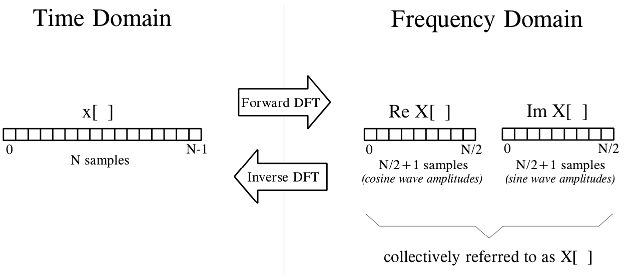
\includegraphics[scale=0.7]{Imagenes/TDF_05.png}
    \caption{Notación y formato de la Transformada discreta de Fourier.}
    \label{fig:figura_TDF_05}
\end{figure}

Se dice que la señal de entrada está en el dominio del tiempo. Esto se debe a que el tipo más común de señal que ingresa a las muestras de DFT se toma a intervalos regulares de tiempo. Por supuesto, cualquier tipo de datos muestreados pueden introducirse en la DFT, independientemente de cómo se adquirieron. Cuando ve el término \enquote{dominio de tiempo} en el análisis de Fourier, en realidad puede referirse a muestras tomadas a lo largo del tiempo, o puede ser una referencia general a cualquier señal discreta que se esté descomponiendo. El término dominio de frecuencia se utiliza para describir las amplitudes de las ondas senoidales y coseno.
\par
El dominio de frecuencia contiene exactamente la misma información que el dominio de tiempo, solo que en una forma diferente. Si conoces un dominio, puedes calcular el otro. Dada la señal del dominio del tiempo, el proceso de cálculo del dominio de la frecuencia se denomina descomposición, análisis, la DFT directa, o simplemente, la DFT. Si conoce el dominio de la frecuencia, el cálculo del dominio del tiempo se denomina síntesis o DFT inversa. Tanto la síntesis como el análisis se pueden representar en forma de ecuaciones y algoritmos computacional.
\par
El número de muestras en el dominio del tiempo generalmente está representado por la variable $N$. Mientras que $N$ puede ser cualquier entero positivo, generalmente se elige una potencia de dos, es decir: $128, 256, 512, 1024$, etc. Hay dos razones para esto:
\begin{enumerate}
\item El almacenamiento de datos digitales utiliza direccionamiento binario, lo que hace que la potencia de dos sea una longitud de señal natural.
\item El algoritmo más eficiente para calcular la DFT, la Transformada Rápida de Fourier \emph{Fast Fourier Transform (FFT)}, generalmente opera con $N$, que es una potencia de dos. Normalmente, $N$ se selecciona entre $32$ y $4096$. En la mayoría de los casos, las muestras se ejecutan de $0$ a $N - 1$, en lugar de $1$ a $N$.
\end{enumerate}
La notación estándar usada en el procesamiento digital de señales utiliza letras minúsculas para representar señales de dominio de tiempo, como $x[ \, ]$, $y[ \, ]$ y $z [ \, ]$. Las letras mayúsculas correspondientes se utilizan para representar sus dominios de frecuencia, es decir, $X[ \, ]$, $Y[ \, ]$ y $Z[ \, ]$. Para ilustrar, supongamos que una señal de dominio de tiempo de punto $N$ está contenida en $x[ \, ]$. El dominio de frecuencia de esta señal se llama $X[ \, ]$ y consta de dos partes, cada una de ellas con una matriz de $N / 2 + 1$ muestras. Estas se denominan la parte real de $X[ \, ]$, escrita como: $\Re X[ \, ]$, y la parte imaginaria de $X[ \, ]$, escrita como: $\Im X[ \, ]$.
\par
Los valores en $\Re X [ \, ]$ son las amplitudes de las ondas del coseno, mientras que los valores en $\Im X[ \, ]$ son las amplitudes de las ondas senoidales (sin preocuparse por el momento, de los factores de escala).
\par
Al igual que el dominio de tiempo se ejecuta de $x[0]$ a $x[N - 1]$, las señales de dominio de frecuencia se ejecutan de $\Re X[0]$ a $\Re X[N / 2]$, y de $\Im X[0]$ a $\Im X[N / 2]$. %Estudia estas notaciones cuidadosamente; Son críticos para entender las ecuaciones en DSP. Desafortunadamente, algunos lenguajes informáticos no distinguen entre mayúsculas y minúsculas, por lo que los nombres de las variables dependen del programador individual. Los programas en este libro utilizan la matriz XX [] para retener la señal de dominio de tiempo, y las matrices REX [] e IMX [] para retener las señales de dominio de frecuencia.
\end{document}
